\documentclass[12pt,a4paper,oneside]{book}
\usepackage[utf8]{inputenc}
\usepackage[spanish]{babel}
\usepackage[T1]{fontenc}
\usepackage{textcomp}
\usepackage[T1]{fontenc}
\usepackage{hyperref}
\usepackage{amsmath}
\usepackage{amsfonts}
\usepackage{amssymb}
\usepackage{graphicx}
\usepackage[utf8]{inputenc}
\usepackage[left=2.54cm, right=2.54cm, top=2.54cm, bottom=2.54cm]{geometry}
\usepackage{tabularx}
\usepackage{listings}[utf8]
\usepackage{xcolor}
\usepackage{makeidx}
\raggedbottom
\makeindex
\date{\today}

\hypersetup{
	colorlinks=true,
	linkcolor=blue,
	filecolor=magenta,
	urlcolor=cyan,
	pdftitle={Overleaft Example},
}
\lstset{inputpath=../}
\lstdefinelanguage{JavaScript}{
  keywords={typeof, new, true, false, catch, function, return, null, catch, switch, var, if, in, while, do, else, case, break},
  keywordstyle=\color{blue}\bfseries,
  ndkeywords={class, export, boolean, throw, implements, import, this},
  ndkeywordstyle=\color{darkgray}\bfseries,
  identifierstyle=\color{black},
  sensitive=false,
  comment=[l]{//},
  morecomment=[s]{/*}{*/},
  commentstyle=\color{purple}\ttfamily,
  stringstyle=\color{red}\ttfamily,
  morestring=[b]',
  morestring=[b]"
}

\lstset{
   language=JavaScript,
   backgroundcolor=\color{lightgray},
   extendedchars=true,
   basicstyle=\footnotesize\ttfamily,
   showstringspaces=false,
   showspaces=false,
   numbers=left,
   numberstyle=\footnotesize,
   numbersep=9pt,
   tabsize=2,
   breaklines=true,
   showtabs=false,
   captionpos=b
}
\definecolor{codegreen}{rgb}{0,0.6,0}
\definecolor{codegray}{rgb}{0.5,0.5,0.5}
\definecolor{codepurple}{rgb}{0.58,0,0.82}
\definecolor{backcolour}{rgb}{0.95,0.95,0.92}

\lstdefinestyle{mystyle}{
	backgroundcolor=\color{backcolour},   
	commentstyle=\color{codegreen},
	keywordstyle=\color{blue},
	numberstyle=\tiny\color{codegray},
	stringstyle=\color{codepurple},
	basicstyle=\ttfamily\footnotesize,
	breakatwhitespace=false,         
	breaklines=true,                 
	captionpos=b,
	keepspaces=true,                 
	numbers=left,                    
	numbersep=5pt,                  
	showspaces=false,                
	showstringspaces=false,
	showtabs=false,                  
	tabsize=4,
	classoffset=1,% starting a new class
	morekeywords={True},
	keywordstyle=\color{red},
	classoffset=6,% starting a new class
	morekeywords={True},
	keywordstyle=\color{green},
	classoffset=0,
}

\usepackage{caption}
\captionsetup[table]{name=Tabla}
\renewcommand*{\lstlistingname}{Exemplo de código}
\renewcommand{\listfigurename}{Figuras}
\renewcommand{\listtablename}{Tablas}

\pagenumbering{arabic}
\lstset{
	style=mystyle,
	inputencoding=utf8,
	extendedchars=true,                    
	literate={á}{{\'a}}1 {ã}{{\~a}}1 {é}{{\'e}}1,
}

%Final Python listing configuration
% Biliografia configuracion
\usepackage[
backend=biber,
style=alphabetic,
sortcites,
url=true
]{biblatex}
\addbibresource{bibliography.bib}
\captionsetup[figure]{labelformat=simple,justification=centerlast}

\begin{document}
	\begin{titlepage}
	\noindent
	\centering
	\Large {Title Book}
	\begin{center}
		\centering
		\rule{150 mm}{0.1 mm}
		\Large {Latex template\\}
		
		\rule{150 mm}{0.1 mm}
		\large {{Description}}
		\rule{150 mm}{0.4 mm}
		\vspace{1 cm}
		\vspace{0.3 cm}
		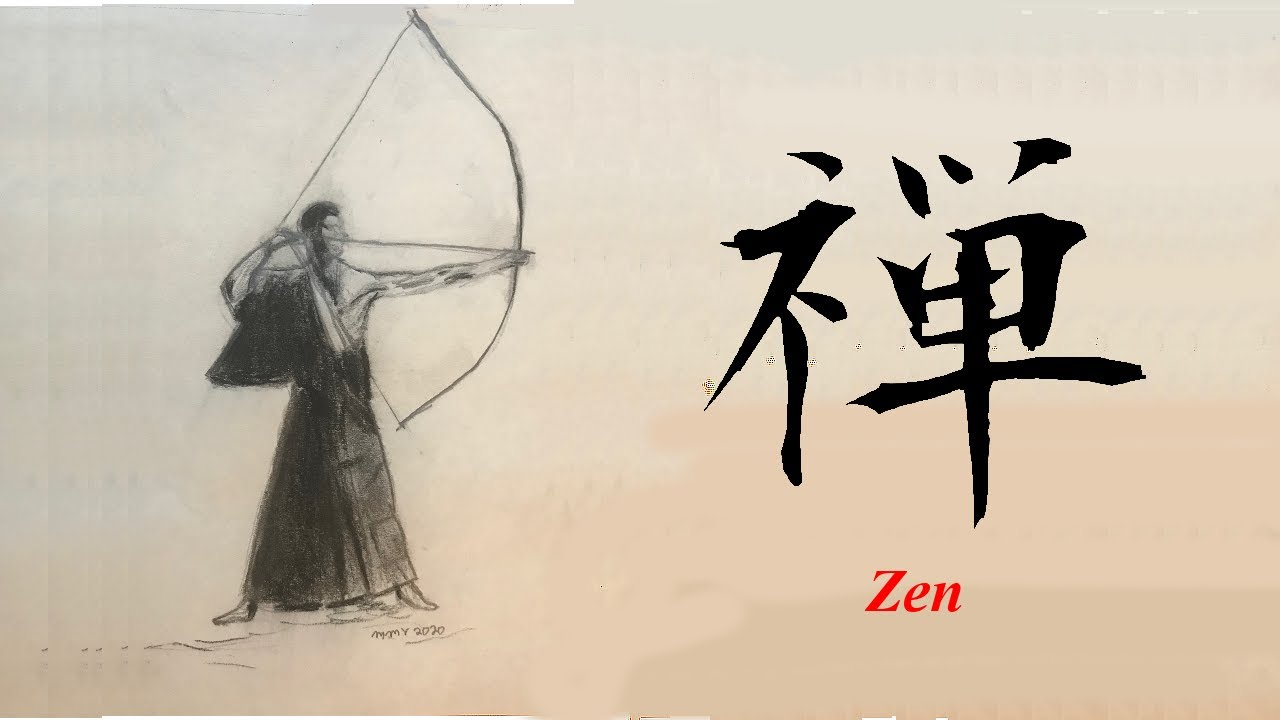
\includegraphics[width=1\textwidth]{image/cover.jpg}
	\end{center}
	\vspace{0.3 cm}
	\begin{center}
		{\large AUTOR
			{\href{https://github.com/titor-oopart/}{@TITOR-OOPART}}}	\\
		{\large YOUTUBE:	{\href{https://www.youtube.com/@ReadToRun}{@ReadToRun}}}	\\
		{\large GITHUB BOOK:  	{\href{https://github.com/titor-oopart/latex_template_book}{@Template-latex-book}}}\\
	\end{center}
	\vspace{0.5 cm}
	\vfill
	\begin{center}
		\large\today
	\end{center}
\end{titlepage}

	\thispagestyle{empty}
	\tableofcontents
	\listoffigures
	\listoftables
	\lstlistoflistings
	\chapter{Example}
Small desctiption \cite{lehman2006biblatex} en la figura \ref{figura1}

\begin{lstlisting}[language=python,caption={Python example}]
def test(name):
	print(name)
\end{lstlisting}
\begin{table}[h]
	\centering
	\begin{tabular}{l | l | l}
		A & B & C \\
		\hline
		1 & 2 & 3 \\
		4 & 5 & 6
	\end{tabular}
	\caption{very basic table}
	\label{tab:abc}
\end{table}

\begin{table}[h]
	\centering
	\begin{tabular}{| l c r |}
		\hline
		1 & 2 & 3 \\
		4 & 5 & 6 \\
		7 & 8 & 9 \\
		\hline
	\end{tabular}
	\caption{A simple table}
\end{table}


\begin{figure}[h]
	
	\centering
	
	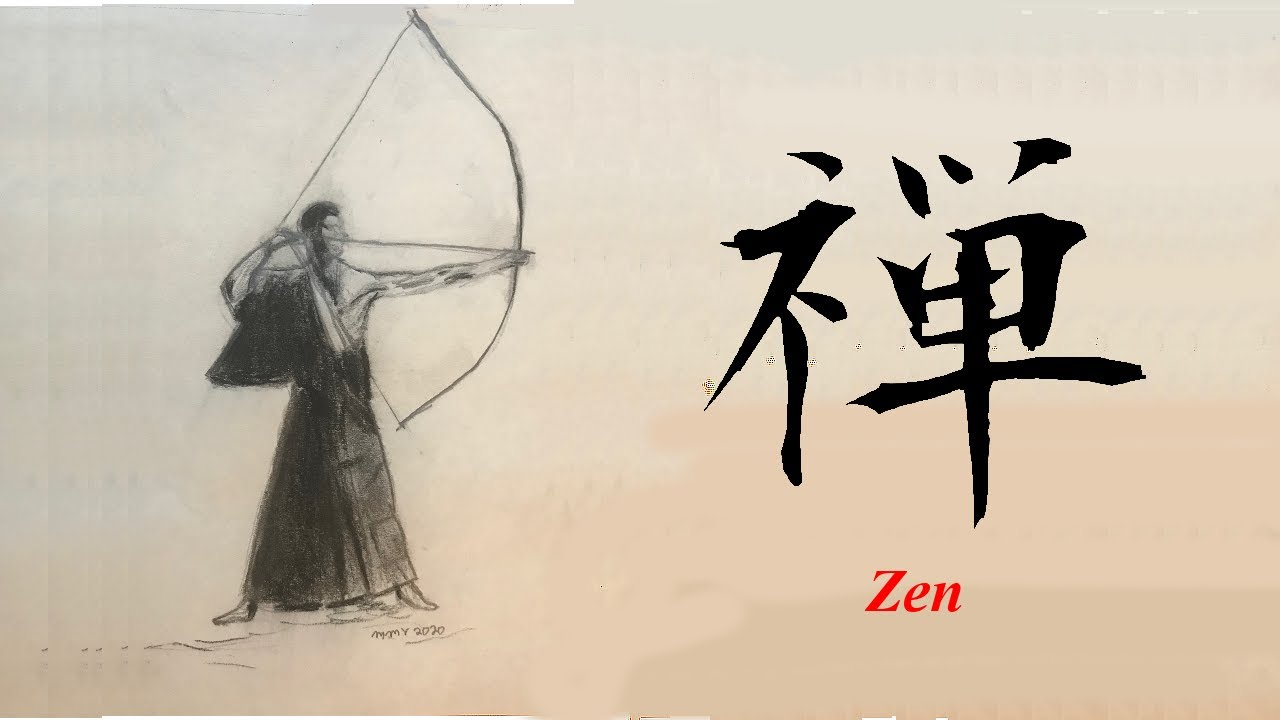
\includegraphics[width=0.5\textwidth]{image/cover.jpg}
	
	\caption{Figure description.}
	
	\label{figura1}
	
\end{figure}
	\chapter{Structure and Data Handling}

%	\chapter{Conditional statements}

%	\chapter{Loops}

%	\chapter{Functions}

%	\chapter{Array and Objects}

%	\chapter{Advanced Functions}

%	\chapter{Debugin and Error Handling}

%	\chapter{Introduction to Document Object Model DOM}

%	\chapter{Events Handling}

%	\chapter{DOM Events}

%	\chapter{Callbacks}

%	\chapter{Promises}

%	\chapter{Async and Await}

%	\chapter{Working with API}

	\printbibliography[heading=bibintoc]
\end{document}
